% TikZ diagrams - current thesis-evidence safe definitions
% These macros intentionally avoid superseded TruthfulQA-only Energy/Cascade claims.

\definecolor{primaryblue}{RGB}{31,119,180}
\definecolor{secondaryorange}{RGB}{255,127,14}
\definecolor{accentgreen}{RGB}{44,160,44}
\definecolor{accentpurple}{RGB}{148,103,189}
\definecolor{neutralgray}{RGB}{127,127,127}
\definecolor{lightgray}{RGB}{200,200,200}
\definecolor{hallred}{RGB}{214,39,40}
\definecolor{normgreen}{RGB}{44,160,44}

% Current method sketch: corpus-grounded selective fusion, with true Energy gated off.
\newcommand{\cascadediagram}{
\begin{tikzpicture}[
    node distance=1.4cm,
    >={Stealth[length=2.5mm]},
    box/.style={rectangle, draw=black!70, line width=0.8pt, rounded corners=2pt,
        minimum width=3.1cm, minimum height=0.9cm, align=center, font=\small},
    source/.style={box, fill=lightgray!30},
    feature/.style={box, fill=primaryblue!15},
    corpus/.style={box, fill=accentgreen!18},
    blocked/.style={box, fill=secondaryorange!18, dashed},
    output/.style={box, fill=accentpurple!15},
    arrow/.style={->, line width=0.8pt, black!70}
]
\node[source] (rows) {feature table\\1000 rows};
\node[feature, right=1.6cm of rows] (se) {SE + cluster count};
\node[corpus, below=1.0cm of se] (corpus) {corpus features\\entity frequency/co-occurrence};
\node[blocked, above=1.0cm of se] (energy) {true Energy unavailable\\\texttt{full\_logits\_required}};
\node[output, right=1.8cm of se] (fusion) {learned fusion\\with/without corpus};
\node[output, right=1.8cm of fusion] (metrics) {AUROC/AUPRC/F1\\current evidence export};
\draw[arrow] (rows) -- (se);
\draw[arrow] (se) -- (fusion);
\draw[arrow] (corpus) -| (fusion);
\draw[arrow, dashed] (energy) -| node[font=\scriptsize, fill=white] {not scored} (fusion);
\draw[arrow] (fusion) -- (metrics);
\end{tikzpicture}
}

% Energy status summary: no thesis-valid Energy AUROC without row-level full logits.
\newcommand{\zerosefigure}{
\centering
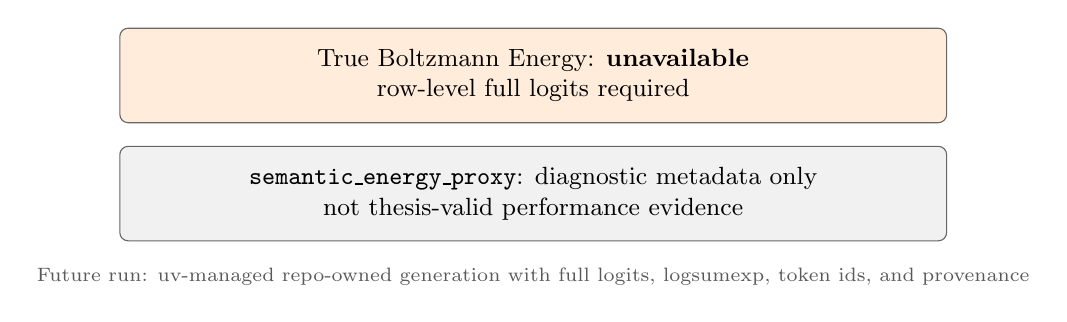
\begin{tikzpicture}[font=\small]
\node[draw=black!60, rounded corners=3pt, fill=secondaryorange!15,
      minimum width=10.5cm, minimum height=1.2cm, align=center] at (0,1.2)
      {True Boltzmann Energy: \textbf{unavailable}\\row-level full logits required};
\node[draw=black!60, rounded corners=3pt, fill=lightgray!25,
      minimum width=10.5cm, minimum height=1.2cm, align=center] at (0,-0.3)
      {\texttt{semantic\_energy\_proxy}: diagnostic metadata only\\not thesis-valid performance evidence};
\node[font=\scriptsize, text=black!65] at (0,-1.35)
      {Future run: uv-managed repo-owned generation with full logits, logsumexp, token ids, and provenance};
\end{tikzpicture}
}

% Current baseline comparison. Energy-dependent baselines are shown as unavailable, not as bars.
\newcommand{\crossoverfigure}{
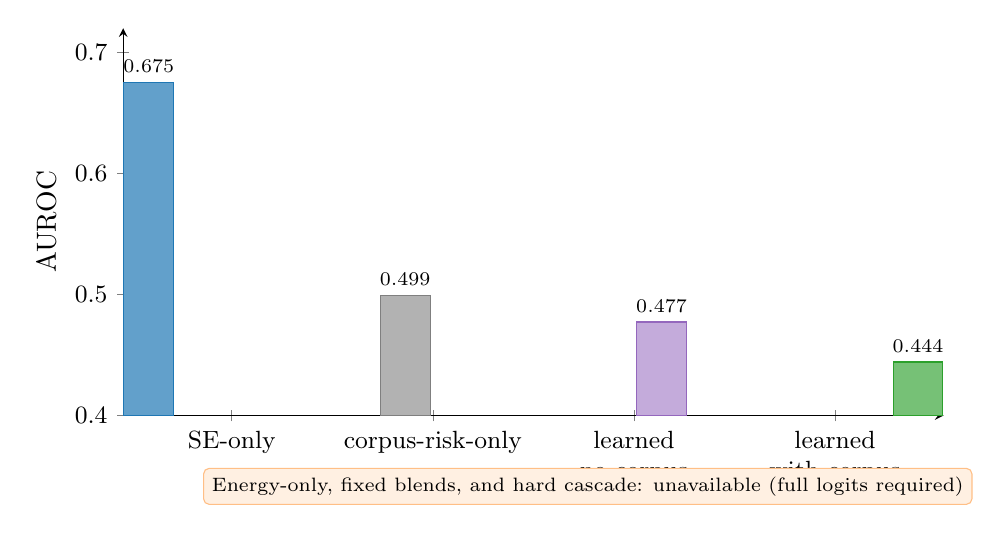
\begin{tikzpicture}
\begin{axis}[
    ybar,
    width=12cm, height=6.5cm,
    bar width=18pt,
    ylabel={AUROC},
    ymin=0.40, ymax=0.72,
    xtick={1,2,3,4},
    xticklabels={SE-only, corpus-risk-only, learned\\no corpus, learned\\with corpus},
    xticklabel style={align=center, font=\small},
    tick label style={font=\small},
    nodes near coords,
    nodes near coords style={font=\scriptsize, /pgf/number format/.cd, fixed, precision=3},
    axis lines=left,
    enlarge x limits=0.18,
]
\addplot[fill=primaryblue!70, draw=primaryblue] coordinates {(1,0.675244)};
\addplot[fill=neutralgray!60, draw=neutralgray] coordinates {(2,0.499133)};
\addplot[fill=accentpurple!55, draw=accentpurple] coordinates {(3,0.477294)};
\addplot[fill=accentgreen!65, draw=accentgreen] coordinates {(4,0.444207)};
\end{axis}
\node[font=\scriptsize, align=center, fill=secondaryorange!12, draw=secondaryorange!50,
      rounded corners=2pt, inner sep=3pt] at (5.9,-0.9)
      {Energy-only, fixed blends, and hard cascade: unavailable (full logits required)};
\end{tikzpicture}
}

% Robustness caveat: corpus learned fusion underperforms on observed AUROC.
\newcommand{\complementarityfigure}{
\centering
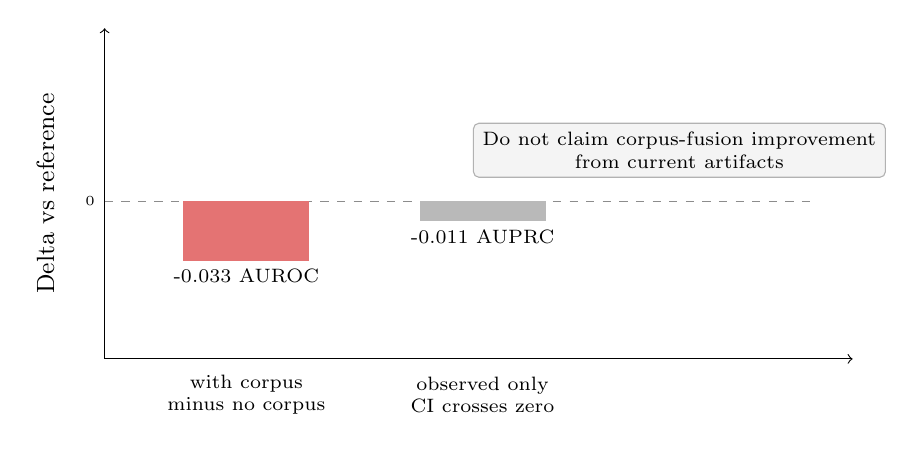
\begin{tikzpicture}[font=\small]
\draw[->] (0,0) -- (0,4.2);
\draw[->] (0,0) -- (9.5,0);
\node[rotate=90, font=\small] at (-0.75,2.1) {Delta vs reference};
\draw[dashed, black!45] (0,2.0) -- (9.0,2.0);
\node[font=\tiny, left] at (0,2.0) {0};
\fill[hallred!65] (1.0,2.0) rectangle (2.6,1.25);
\node[font=\scriptsize] at (1.8,1.05) {-0.033 AUROC};
\node[font=\scriptsize, align=center] at (1.8,-0.45) {with corpus\\minus no corpus};
\fill[neutralgray!55] (4.0,2.0) rectangle (5.6,1.75);
\node[font=\scriptsize] at (4.8,1.55) {-0.011 AUPRC};
\node[font=\scriptsize, align=center] at (4.8,-0.45) {observed only\\CI crosses zero};
\node[draw=black!30, rounded corners=2pt, fill=lightgray!20, align=center,
      font=\scriptsize, minimum width=3.2cm] at (7.3,2.65)
      {Do not claim corpus-fusion improvement\\from current artifacts};
\end{tikzpicture}
}

% Overall current evidence figure: no Energy/Cascade AUROC bars.
\newcommand{\overallfigure}{
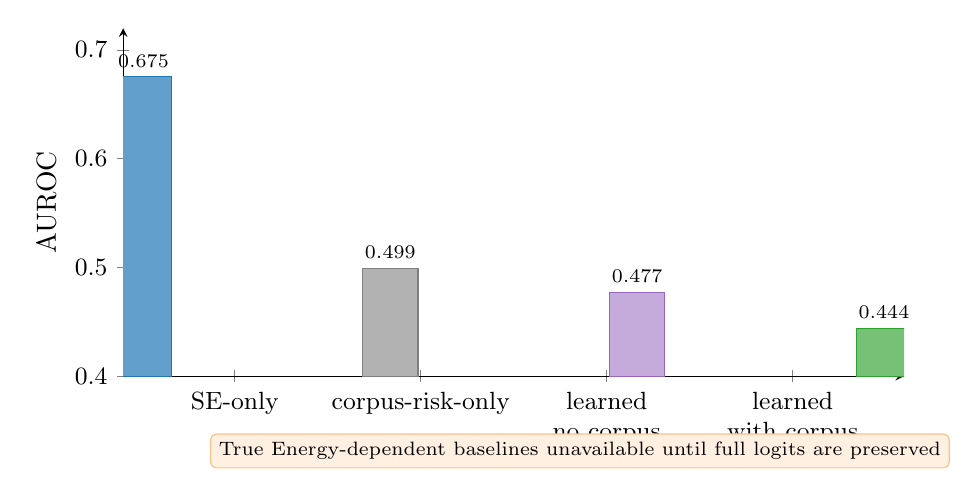
\begin{tikzpicture}
\begin{axis}[
    ybar,
    width=11.5cm, height=6cm,
    bar width=20pt,
    ylabel={AUROC},
    ymin=0.40, ymax=0.72,
    xtick={1,2,3,4},
    xticklabels={SE-only, corpus-risk-only, learned\\no corpus, learned\\with corpus},
    xticklabel style={align=center, font=\small},
    tick label style={font=\small},
    nodes near coords,
    nodes near coords style={font=\scriptsize, /pgf/number format/.cd, fixed, precision=3},
    axis lines=left,
    enlarge x limits=0.2,
]
\addplot[fill=primaryblue!70, draw=primaryblue] coordinates {(1,0.675244)};
\addplot[fill=neutralgray!60, draw=neutralgray] coordinates {(2,0.499133)};
\addplot[fill=accentpurple!55, draw=accentpurple] coordinates {(3,0.477294)};
\addplot[fill=accentgreen!65, draw=accentgreen] coordinates {(4,0.444207)};
\end{axis}
\node[font=\scriptsize, align=center, fill=secondaryorange!12, draw=secondaryorange!50,
      rounded corners=2pt, inner sep=3pt] at (5.8,-0.95)
      {True Energy-dependent baselines unavailable until full logits are preserved};
\end{tikzpicture}
}
